\documentclass[12pt,a4paper]{article}

\usepackage[pdftex]{graphicx}
\usepackage{amsmath}
\usepackage{amsopn,amscd,amsthm,amssymb,xypic,rotating}
\usepackage{thmtools}
\usepackage[utf8]{inputenc}
\usepackage{changebar}
%\usepackage[dvinames]{xcolor}
\usepackage{mathtools}
\usepackage{hyperref}

\newcommand{\tset}[1]      {\{{#1}\}}                     % set data type
\newcommand{\tbag}[1]      {\{\!\!|{#1}\}\!\!\!|}         % bag data type
\newcommand{\tlist}[1]     {[{#1}]}                       %list data type
\newcommand{\ttree}[1]     {{\frak t}({#1})}              %tree data type
\newcommand{\cmd}[1]      {\underline{{#1}}}
\newcommand{\cb}          {\begin{tabbing}MMMMM\=MM\=MM\=MM\=MM\=MM\=MM\=MM\=MM\=MM\= \kill}
\newcommand{\ce}          {\end{tabbing}}
\newcommand{\ontology}[1]	{\ensuremath{\mathcal{#1}}}
\newcommand{\ont}[1]	{\ontology{#1}}
\newcommand{\conceptualization}[1]	{\ensuremath{\mathcal{#1}}}
\newcommand{\conc}[1]	{\conceptualization{#1}}

\newcommand{\HInsert}[2]   {\centerline {\immediate\pdfximage width #2  {#1}\pdfrefximage\pdflastximage}}
\newcommand{\VInsert}[2]   {\centerline {\immediate\pdfximage height #2 {#1}\pdfrefximage\pdflastximage}}


%\newtheorem{definition}{Definition}[section]
%\newtheorem{proposition}{Proposition}[section]
%\newtheorem{corollary}{Corollary}[section]
%\newtheorem{theorem}{Theorem}[section]
%\newtheorem{lemma}{Lemma}[section]
%\newtheorem{statement}{Statement}[section]
%\newtheorem{assumption}{Assumption}[section]
%\newtheorem{problem}{Problem}[section]
%\newtheorem{hypothesis}{Hypothesis}

\newcounter{remark}
\newcounter{example}
\setcounter{remark}{0}
\setcounter{example}{0}

\def\example{
\bigskip

\addtocounter{example}{1}%
\noindent \textbf{Example \Roman{example}:}\\
}


\def\remark{
%\addtocounter{remark}{1}%
\refstepcounter{remark}
\noindent \emph{Remark \arabic{remark}:}
}

\renewcommand{\topfraction}{.99}
\renewcommand{\textfraction}{.01}

\newcommand{\dblquote}[1] {\textquotedblleft #1\textquotedblright}

\usepackage{listings}
\usepackage{color}
\usepackage{soul}
\usepackage{etoolbox}

\definecolor{dkgreen}{rgb}{0,0.6,0}
\definecolor{gray}{rgb}{0.5,0.5,0.5}
\definecolor{mauve}{rgb}{0.58,0,0.82}
\definecolor{lightgray}{rgb}{0.7,0.7,0.7}

\lstset{frame=tb,
  language=Prolog,
  aboveskip=3mm,
  belowskip=3mm,
  showstringspaces=false,
  columns=flexible,
  basicstyle={\small\ttfamily},
  numbers=none,
  numberstyle=\tiny\color{gray},
  keywordstyle=\color{blue},
  commentstyle=\color{dkgreen},
  stringstyle=\color{mauve},
  breaklines=true,
  breakatwhitespace=true,
  tabsize=3
}

\newcommand{\mfunc}[1]      {{\it{#1}}}
\newcommand{\mmfunc}[1]      {\text{\it{#1}}}
\newcommand{\defining}[1] {\emph{#1}}
\newcommand{\keyconcept}[1] {\emph{#1}}
\newcommand{\takeaway}[1] {{\bf{#1}}}
\newcommand{\itemtitle}[1] {{\bf{#1}} - }

\newcommand{\metavars}[1] {\mathcal{#1}}
\newcommand{\unsatmap} {\rightarrow^{\mmfunc{unsat}}}

\newcommand{\objectvar}[1] {\lowercase{#1}}
\newcommand{\metavar}[1] {\uppercase{#1}}
\newcommand{\metametavar}[1] {\mathcal{\uppercase{#1}}}

\newtoggle{annotations}
\toggletrue{annotations}

\newcommand{\noannotations}[0] {\togglefalse{annotations}}

\newcommand{\annotation}[1] {\iftoggle{annotations}{\sethlcolor{lightgray}\hl{#1}}{}}

\def\entails{\mathrel{\vDash}}
\def\satisfies{\mathrel{{\vDash}^{*}}}
\def\entailsf{\mathrel{!\entails}}
\def\satisfiesf{\mathrel{!\satisfies}}
\def\runafter{\mathrel{\overleftarrow{\cup}}}

\def\unsatisfies{\mathrel{\not\satisfies}}
\def\unentails{\mathrel{\not\entails}}
\def\unsatisfiesf{\mathrel{!\unsatisfies}}
\def\unentailsf{\mathrel{!\unentails}}

\def\mbsatisfies{\mathrel{?\satisfies}}

\def\dirreduce{\rightarrow}
\def\indreduce{\overset{i}\rightarrow}
\def\reduce{\overset{*}\rightarrow}
\def\syneq{\equiv}
\def\semeq{\cong}
\def\subeq{\approx}
\newcommand{\normform}[1] {\mathcal{N}(#1)}
\newcommand{\normlevel}[1] {\mathcal{N}^{#1}}
\newcommand{\rulenormlevel}[1] {\mathcal{R}^{#1}}
\newcommand{\uniflevel}[1] {\bar{\sigma}(#1)}
\def\finer{\preceq}
\def\stfiner{\prec}
\def\foproxy{\kappa}
\def\soproxy{\chi}
\newcommand{\depgraph}[1] {\mathcal{#1}}
\newcommand{\depgraphset}[1] {\mathbb{#1}}
\newcommand{\eqsys}[1] {\mathcal{E}(#1)}
\newcommand{\usols}[1] {\mathcal{U}(#1)}
\def\eqeq{\simeq}
\newcommand{\measure}[1] {\mu^{#1}}
\newcommand{\depbdryone}[1] {\mathcal{D}^1(#1)}
\newcommand{\depbdrytwo}[1] {\mathcal{D}^2(#1)}
\newcommand{\searchtree}[1] {\mathcal{#1}}
\newcommand{\leaves}[1] {\mathcal{L}(#1)}
\def\diagonalize{\mathbb{D}}

\newcommand\Wider[2][3em]{%
\makebox[\linewidth][c]{%
  \begin{minipage}{\dimexpr\textwidth+#1\relax}
  \raggedright#2
  \end{minipage}%
  }%
}

%\tikzstyle{myellipse} = [draw=black, ellipse,align=center]
%\tikzstyle{myrectangle} = [draw=black, rectangle,align=center]

\newtheorem{conjecture}{Conjecture}

\title{BiRating - Iterative averaging on a bipartite graph of Beat Saber scores, player skills, and map difficulties}
\author{Juan Casanova}

\begin{document}

\maketitle

Abstract here

\tableofcontents

\section{Introduction}

Beat Saber\footnote{\url{https://beatsaber.com/}} is a virtual reality rhythm game developed by Beat Games and released in 2018. Players play {\emph{maps}} of {\emph{songs}} that present the player with notes timed to and representing the music that they must cut in specific directions to score, among other gameplay mechanics. Maps for faster songs often have faster patterns that require the player to react more quickly, and other maps have more complex patterns that are more difficult to understand and play. Beat Saber has rich scoring mechanics\footnote{\url{https://bsmg.wiki/ranking-guide.html}}, and a healthy competitive scene with upwards of 60 thousand active ranked players in the second half of 2024\footnote{Verified using BeatLeader's search functionality at \url{https://beatleader.com/ranking/1?mapsType=all&recentScoreTime=1721433600}}, which can be observed through its two most important ranked leaderboards: ScoreSaber\footnote{\url{https://scoresaber.com/}} and BeatLeader\footnote{\url{https://beatleader.xyz/}}. Competitive Beat Saber focuses on large pools of {\emph{custom}} maps made by members of the community ({\emph{mappers}}) that undergo a ranking process\footnote{\url{https://beatleader.wiki/en/ranking/Ranking-your-map}} to ensure their competitive viability. For example, as of January 2025, BeatLeader offers over 3500 different ranked maps\footnote{\url{https://beatleader.xyz/leaderboards}}.

Because of the diversity of maps and map difficulty, a key question that ranking leaderboards need to address is: {\emph{How do you compare scores on different maps to determine which one indicates a higher player skill?}} This question is normally reduced to the question of quantifying the difficulty of a map. In general, there is an understanding in the ranked community that Beat Saber skill is not unidimensional, with different players possessing different playstyles and skillsets that allow them to perform better at some maps and worse at others. For example, {\emph{speed}} players will perform well on fast but simple ({\emph{speed}}) maps, where {\emph{tech}} players will perform well on complex but slower ({\emph{tech}}) maps. However, due to the large dimensionality of the variety in maps and playstyles, the problem of accurately quantifying difficulty of maps is complex and not completely understood.\\

ScoreSaber and BeatLeader each use their own machine learning / hybrid algorithms to calculate the difficulty ratings of maps. For example, BeatLeader calculates three different ratings on each map, based on the placement of notes and other objects in the map, each of which contributes in a different way to PP (a measure of how good a certain score on a certain map is):

\begin{itemize}

\item \itemtitle{Pass rating} Indicates how difficult the map is to pass (play without failing). This gives a flat PP to any player that passes the map.
\item \itemtitle{Tech rating} Indicates how complex the map is, especially in terms of the difficulty in understanding it ({\emph{reading it}}). This gives a small amount of PP based on the score the player obtained in the map.
\item \itemtitle{Acc rating} Indicates how difficult it is to achieve a high score (acc) on each of the individual notes of the map, based on their positioning, angle, and context. This gives the majority of the PP obtained by the player, depending on the score the player obtained in the map.

\end{itemize}

Pass and Tech rating are calculated based on rules\footnote{\url{https://github.com/LackWiz/ppCurve}}, while Acc rating uses custom neural networks trained on replays of good players on ranked maps to predict the score that players will likely obtain on each of the individual notes in the map based on their context and parameters\footnote{\url{https://github.com/BeatLeader/beatsaber-replays-ai-2} or \url{https://github.com/DziugasRam/bs-replays-ai-api}}.\\

Iterative algorithms on graph data structures to extract underlying knowledge are widely used \cite{survey_distributed_graph_pattern_matching, survey_distributed_graph_algorithms}. This paper describes a novel iterative averaging algorithm on the graph of maps, players, and scores, to estimate the difficulty of maps and the player skill of players simultaneously based entirely on the relative scores of different players on different maps. More specifically, we can define a bipartite graph with maps and players as the two classes of nodes, and edges representing the best score of the player on that map. This graph allows us to consider the direct relation between multiple scores by different players on the same map, between multiple scores by the same player on different maps, and the transitive relations that can be inferred from this. Conceptually, this graph contains enough information to determine both which maps are more difficult, and which players are better. We need only to extract it. We designed, implemented, and evaluated an iterative averaging algorithm that does this.\\

This approach is different to previous attempts to quantify difficulty in Beat Saber maps primarily in that it utilizes scores exclusively to determine difficulty, rather than note and object placement in the map. This means both that the algorithm uses a significantly smaller amount of data to train, and that it may focus exclusively on the observed patterns of difficulty in the scores by different players to quantify and compare more objectively the relative difficulty of maps. However, it also means that the applicability of the algorithm has a number of important limitations, discussed in \S \ref{limitations}. Furthermore, this algorithm is unsupervised, using observations of scores to estimate skills and difficulties, rather than requiring labelled data about skills or difficulties.

This approach is different to other iterative averaging algorithms in bipartite graphs \cite{consensus_bipartite_graphs, iterative_algorithm_priority_pairwise, averaging_process_bipartite_graphs} in the particularities of the mathematical problem. In particular, in this problem there is a tension between player skills and map difficulties, where a better score could be explained {\emph{either}} by an easier map or a better player, and a better player skill increases the perceived difficulty of the map, and viceversa. More importantly, the edges (scores) on the graph do not represent a strength of the relation between players and maps, but rather an observation that needs to be explained and can be explained in multiple ways. In typical recommender systems and other problems for which iterative averaging algorithms are used, the underlying situation is one of similarities and relatedness. But in this problem, all players, including high skill players, will obtain better scores on easier maps, and a better player will obtain better scores on all maps. In other words, higher values of the edges (scores) do not represent a stronger connection between the nodes, merely an observation to be explained. This drastically changes the underlying  maths, but can still be approached using an iterative averaging algorithm.\\

The remainder of this document is structured as follows.

\begin{itemize}

\item Section \ref{algorithm_description} describes the mathematical principles of the algorithm and some of its properties.
\item Section \ref{data_preparation_implementation} explains the data preparation conducted for this work and relevant details about the implementation of the algorithm.
\item Section \ref{results} presents, discusses, and evaluates the results of the implementation of the algorithm in terms of its ability to produce a good estimation of map difficulty.
\item Section \ref{limitations} discusses the most important known limitations of this approach.
\item Section \ref{related_future_work} discusses some related and future work and its relation to the work presented in this document.
\item Finally, section \ref{conclusions} offers some general conclusions.

\end{itemize}

\section{Algorithm description}
\label{algorithm_description}

This section describes the core conceptual and mathematical principles behind the algorithm. The actual implementation details, along with additional choices and manipulations of the data that were carried out in practice, and their motivation, are explained in \S \ref{data_preparation_implementation}. Here, we stick to the main idealized aspects.\\

\subsection{Bilinear relationship between player skills, map ease, and scores}

The core principle of the algorithm is to define a relationship between {\emph{player skill}} ($p$), {\emph{map difficulty}}, and {\emph{scores}} ($s$). This allows us to calculate the estimated value of any of these three values if we are given the other two. In order to simplify the maths, we replace map difficulty with map {\emph{ease}} ($e$), which can be seen as the inverse of difficulty: a map with higher ease is easier to score well in. We use a simple bilinear relationship between these to enable iterative averaging to work well.\\

\begin{equation}
\label{bilinear_relation}
s = p \cdot e
\end{equation}

For example, if a player has player skill $p = 1.5$ and a map has ease $e = 0.5$, we expect that player to set a score with value $s = 1.5 \cdot 0.5 = 0.75$ on that map. We can also work the formula backwards, for example, if a map has ease $e = 0.25$ and a player sets a score with value $s = 1$ on it, this gives us an estimation of that player's skill as $p = s / e = 1 / 0.25 = 4$.\\

\subsection{Ensuring linearity of values}

The assumption of bilinearity is mainly for simplicity purposes, and is important for the success of the algorithm, though we expect that other kinds of relationships could also be made to work in similar algorithms. More important is the right choice of the representation of player skill, map ease, and score values. Our data consists of map scores in Beat Saber. While there are multiple ways to represent this, the typical way in which the Beat Saber community looks at them is also useful for our purposes: the score is a percentage representing what proportion of the maximum possible score on a map the player obtained. We will represent this as a value between 0 and 1. 

However, the distribution, and more importantly, the perception of difficulty of scores is far from being uniformly distributed across the $[0,1]$ interval. Here are some general ranges of expected scores:

\begin{itemize}

\item Scores below 0.5 almost universally denote a fail on the map and are extremely poor.
\item A score of 0.8 is still considered relatively poor and most players can achieve this on maps that are approachable to them.
\item A score of 0.9 indicates a decent play depending on the difficulty of the map but for most maps, many players will be able to achieve this.
\item A score of 0.96 is often seen as the gold standard of a good play, with anything above it being a significantly good play. While this definitely depends on the map, 0.96 is frequently seen as the inflection point where increasing score becomes significantly more difficult.
\item A score of 0.98 is very difficult to achieve even on the easiest maps and only the best players are able to reach this even on the simplest maps.
\item A score of 0.99 is extremely high and only the best players on the easiest maps with a lot of practice and iteration can achieve such scores.
\item There is only a single score of 1 (100\%) in the entirety of the ranked leaderboards in BeatLeader, by a high level player on what is considered to be the easiest ranked map.

\end{itemize}

This perception can be visualized in the way in which the current BeatLeader algorithm rewards scores on maps, also known as ``the PP curve''. See figure \ref{PP_curve}.

\begin{figure}
\label{PP_curve}
\caption{BeatLeader's PP curve on a ranked map.}
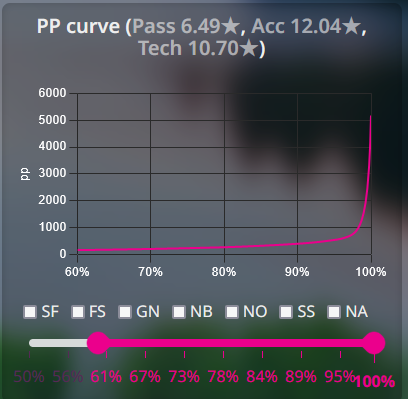
\includegraphics[width=0.5\textwidth]{PPcurve.png}
\centering
\end{figure}

In order to make our bilinearity assumption work well, we need a way to value scores, skills, and map ease that is linear. Therefore, we need to transform the percentage scores into a different representation that behaves more linearly. Since the score on a map is between 0 and 1 and the value of a play is monotonically increasing, it makes sense to look at it as a probabilistic distribution and use the inverse of the cumulative distribution to estimate the value of the score. Moreover you can interpret a score on a map as the probability of making fewer than a certain number of mistakes in the map. We discuss this approach further and the explicit formulas that we considered and implemented to transform scores into score values in \S \ref{data_preparation_implementation}. For this section, we merely state that the score value $s$ will be calculated in such a way from the scores on maps that it is as close to linear as possible. That is, that a score value that is double of another will represent a twice as valuable score.

We do not need to make any such assumption for player skills or map ease, as we do not use any reference scale for these. We use the score values to estimate player skill and map ease values, and therefore the scaling of the scores will be the one to determine the scaling of map ease and player skill.\\

\subsection{Iterative averaging}

Another core principle of the algorithm is {\emph{iterative averaging}}. If we have an estimation of map ease for each map and know the value of the scores that a certain player has set, we can estimate that player's skill as the average of the estimated skill that each of those scores represents.

\begin{equation}
\label{player_skill_averaging}
\bar{p}  = {{1} \over {n}} \sum\limits_{i = 1}^{n} {{s_i} \over {e_i}}
\end{equation}

Conversely, if we have an estimation of player skill for each player and know the value of the scores on a certain map, we can estimate thata map's ease as the average of the estimated ease that each of those scores represents.

\begin{equation}
\label{map_ease_averaging}
\bar{e}  = {{1} \over {n}} \sum\limits_{i = 1}^{n} {{s_i} \over {p_i}}
\end{equation}

The algorithm works by alternating averaging steps of each of these two kinds, updating player skils and map ease based on the scores and their relations to each other.\\

\subsection{Error}

One of the desired properties of this algorithm is that the accuracy of the player skills and map ease will increase with each iteration. In order to discuss this at all, we need to usefully define the accuracy of a certain set of values. Given a set of estimations of player skill and map ease values, we can consider what scores those would predict and compare them with the actual scores we observed. We call this the {\emph{error}} of each of the scores, and then define the error of the model to be the mean absolute error of the error of each score $s$ that a player with skill $p$ set on a map with ease $e$.\\

\begin{equation}
\label{error}
\epsilon(s) = |s -  p \cdot e|
\end{equation}

And the average error of the model:

\begin{equation}
\label{average_error}
\bar{\epsilon} = \sum\limits_{i=1}^{n} \epsilon(s_i)
\end{equation}

There are a few important implicit choices here. First, we note that we use the mean absolute error (MAE) rather than the root mean square error (RMSE) or other similar measures. This is because the error of our model is exclusively an evaluation metric and not an explicit goal of the algorithm, and therefore we do not care about its smoothness properties, which is one of the main reasons to favour RMSE over MAE. However, using the RMSE could make sense as well, for example, to give more weight to outliers with large errors. Ultimately this choice can be exchanged with only moderate consequences in, for example, the optimization of model hyperparameters, and is not a core element affecting the algorithm itself. Second, we do not measure the error in proportion to the value of the score, or mean relative error (MRE). Arguably this could make scores with larger values have more relevance to the error. However, there are two reasons why we favour the MAE: it preserves the linear properties that our general model for relationship between skills, ease, and scores has; and due to the domain problem, it makes sense to give higher value scores have a larger role in evaluating and optimizing the algorithm thatn small value scores. Competitiveness focuses primarily on the top players achieving the top scores, and we care more about getting those right. However, similar to RMSE, MRE could also be a reasonable metric to evaluate the algorithm under a different scope.\\

A good measure of the correct working of the algorithm would be that the MAE is reduced on each iteration. We discuss the theoretical aspects around this in \S \ref{convergence} and the results in our implementation in \S \ref{results}.

\subsection{Convergence}
\label{convergence}

Ideally, we would want theoretical proof that the iterative averaging of player skill and map ease values is convergent to a minimum error state. Plenty of results on similar iterative averaging problems follow similar structures \cite{convergence_speed_distributed_consensus,averaging_improve_convergence,average_convergence_iterative_projection,iterative_averaging_saddle_point_problems}. However, we have been unable to find general results that we were  able to apply to our problem. Moreover, our experimental results explained in \S \ref{results} seem to indicate that the method does not exactly converge to a minimum error state. However, there are still some properties of the process, both theoretical and empirically observed, that are relevant to discuss, as well as highlight the theoretical conditions that we are aware would affect this result.\\

First, we note that any state of the model in which all score predictions are perfect ($\bar{\epsilon} = 0$) is a fixed point. This is trivial because if all score predictions are perfect, then the predicted score for each map will be exactly the observed scores, and because we are using the same formula to update estimated player skill and map ease values, for each of these scores, the predicted player skill value will be exactly the current player skill value, and similarly for map ease values. Therefore, the update will not change any values and will remain fixed.

However, in practice it is highly unlikely that an observed dataset will have such a possible state to begin with. It is enough that two players achieved reversely ordered scores on two different maps to ensure that it is not possible to find a fixed point of the system with $\bar{\epsilon} = 0$.\\

We can consider the minimum possible error that a set of observed scores can have within all possible estimations of player skill and map ease values\footnote{Note that the space of possible player skill and map ease values is compact and therefore it will contain a minimum.}. Write ${\bar{\epsilon}}_{\min}$. It would be reasonable to expect that a state with minimum error would be a fixed point. The intuitive argument is that the iteration is doing a best attempt at finding the best way to explain the scores by using averages, and therefore it does not seem expected to have the process increase the error. However, we have not found a theoretical proof of this. Moreover, as described in \S \ref{results}, the empirical process seems to consistently enter a post-optimization regime in which the error slowly increases\footnote{Although there may be other implementation-specific explanations for this phenomenon.}. We cannot at the present  time offer a satisfactory and complete explanation of the reasons behind this, but we conjecture that when certain sets of scores are relevantly incompatible, the iterative averaging may enter an oscillatory and divergent process by which each iteration overcompensates the error on some scores by increasing the error on others. Nonetheless, the process still empirically behaves as convergent, but does not converge to a minimum error state, though it does to a low error state.\\

More in general, we have not been able to prove the existence of fixed points for every set of possible scores, or characterize the conditions on the set of scores that would guarantee the existence of fixed points, nor the contractiveness of the iterative process, which would be conditions for the most likely to work approach to proving convergence of the process (the Banach fixed-point theorem). Conceptually, it would be reasonable to expect that a method based on averaging would be contractive, as it explicitly moves the system towards more regularized states, though it is possible that it has an oscillatory component. Empirical results are more promising, though, and are discussed in \S \ref{results}.\\

To be precise, we have empirical evidence (but no proof) for the following {\bf{conjectures}}:

\begin{itemize}
\item The process is always convergent.
\item The process converges to a low error state.
\item The differences between the fixed points and the minimum error states are caused by inherent incompatibilities between scores  that cause small scale oscillations.
\end{itemize}

\subsection{Summary}

\begin{itemize}

\item We define a bilinear relationship between player skills, map ease, and scores defined by equation \ref{bilinear_relation}.

\begin{equation*}
s = p \cdot e
\end{equation*}

\item We ensure linear behaviour of the values by re-scaling scores using probability distribution interpretations of them.

\item We apply iterative mutual averaging to estimate player skill and map ease values, based on each other and using the observed scores, following equations \ref{player_skill_averaging} and \ref{map_ease_averaging}.

\begin{equation*}
\bar{p}  = {{1} \over {n}} \sum\limits_{i = 1}^{n} {{s_i} \over {e_i}}
\end{equation*}

\begin{equation*}
\bar{e}  = {{1} \over {n}} \sum\limits_{i = 1}^{n} {{s_i} \over {p_i}}
\end{equation*}

\item We use mean absolute error to evaluate the results of the processs and observe its convergence properties. These are defined by equations \ref{error} and \ref{average_error}.

\begin{equation*}
\epsilon(s) = |s -  p \cdot e|
\end{equation*}

\begin{equation*}
\bar{\epsilon} = \sum\limits_{i=1}^{n} \epsilon(s_i)
\end{equation*}

\item While we have not been able to prove convergence, we have investigated the conditions and phenomena that may be affecting the convergence conditions. The process empirically exhibits convergent behaviour towards low error values, though they are not minimum error values.

\end{itemize}

\section{Data preparation and implementation}
\label{data_preparation_implementation}

Implementation details, data preparation, what data I have, what did I do.
Talk about hyperparameter search

\section{Results}
\label{results}

Actual results, direct discussion and its meaning. Talk about convergence again.

Evaluation of results compared to star rating algorithm and community discussion.

\section{Limitations}
\label{limitations}

Inherent algorithm limitations: Convergence.

Data limitations: Data quality, need scores, abuse, not suitable for live system, which scores to pick, irregularity of scores.

Application limitations: Multidimensionality of skill and difficulty, curve shape matters.

\section{Related and future work}
\label{related_future_work}

ALS and other more advanced algorithms.

Mention existing approaches again.

Pattern recognition with neural networks: Supervised data issue, and what is authoritative. Feature selection. Data preprocessing. Curve shape estimation. 

\section{Conclusions}
\label{conclusions}

Interesting approach. Why it is interesting compared to other approaches. Works to some degree. Limitations. More work needed. Helped identify some core difficulties with the approach.

\bibliographystyle{plain}
\bibliography{bibliography}

\end{document}